\documentclass[12pt,a4paper]{article}
\usepackage{fontspec}\defaultfontfeatures{Ligatures=TeX}
\setmainfont{TeX Gyre Termes}\setmonofont{Latin Modern Mono}
\usepackage{amsmath,amssymb,graphicx,float,caption,xcolor,hyperref,fancyhdr,geometry,booktabs,tabularx,tikz}
\usetikzlibrary{positioning,arrows.meta,shapes.geometric}
\geometry{margin=0.9in}\setlength{\headheight}{15pt}
\pagestyle{fancy}\fancyhf{}\lhead{IEEE 14-bus with controller}\rhead{\thepage}
\hypersetup{colorlinks=true,linkcolor=blue!55!black,urlcolor=blue!55!black}
\newcommand{\code}[1]{\texttt{\detokenize{#1}}}
\newcommand{\vect}[1]{\boldsymbol{#1}}
\title{\textbf{IEEE 14-Bus with Controller}\\
\large Production 160-s Comparison of the Legacy Selector, ET-FCSPS, and Finite-Set BO Replay}
\author{In-house Power-Flow Project}\date{4 August 2026}
\begin{document}\maketitle
\begin{abstract}
Three controller arms were evaluated on the same project-owned all-KCL IEEE 14-bus simulation. Case data, initial state, SG/IBR equations, event chronology, dispatch, synchronizer, solver, tolerances, and the fixed $0.0125$-s step were identical. The legacy selector, exhaustive event-triggered finite-control-set predictive supervisor (ET-FCSPS), and finite-set Bayesian-optimisation (BO) replay all selected IBR1--IBR4 as GFM with IBR1 as the island reference owner. All runs reached 160 s and their raw trajectories were numerically identical. In this four-IBR case ET-FCSPS is preferable: only eight candidates pass the authenticated pre-screen, while the frozen BO budget is also eight, so BO provides no evaluation reduction or response improvement.
\end{abstract}

\section{Controller contract}
AGSI++ and authenticated events trigger an evaluation; they do not directly select the mode vector. Every admissible candidate starts from the same accepted event-left state and receives the same SG-trip transaction, device-owned state transfer, post-trip dispatch, full-KCL right-limit solve, and $T_p=0.25$ s production-kernel prediction. Hard KCL, voltage, frequency, RoCoF, current, reserve, dwell, lockout, online-resource, and reference-continuity gates precede the cost
\begin{equation}J=\sum_k w_k\phi_k.
\end{equation}
The terms cover voltage, frequency, RoCoF, P/Q reserve, current utilisation, handback mismatch, GFM count, and switching count. Weights and normalisers were frozen before closed-loop results.

The SG uses the operational sixth-order EMF state
\begin{equation}\vect{x}_{SG}=[\delta,\Delta\omega,E'_q,E'_d,E''_q,E''_d]^T,
\qquad 2H\dot{\Delta\omega}=P_m-P_e-D\Delta\omega.
\end{equation}
Each dual-mode IBR retains a 13-state GFM subset and a 7-state GFL subset. The supervisor changes only the discrete active subset and reference-owner metadata; it does not modify device equations.

\section{BO comparator}
BO is an \textbf{offline finite-set replay} over the identical immutable trial table. It uses an in-house RBF Gaussian process and Expected Improvement,
\begin{equation}
k(\vect{z},\vect{z}')=\exp\left(-\frac{\|\vect{z}-\vect{z}'\|^2}{2\ell^2}\right),
\end{equation}
with a frozen budget of eight. It does not call an external optimiser and is not presented as an online production authority.

\section{Common 160-s experiment}
The chronology is SG trip at 20 s, 20\% load increase at 50 s, bus-9 fault from 85 to 85.15 s, line 6--13 trip at 110 s, and restoration/reclose request at 145 s. The SG passes its synchronism guard at 147.175 s, after which the coordinated reference handback returns all IBRs to GFL.

\begin{table}[H]\centering\caption{Raw production results}\small
\begin{tabular}{lrrr}\toprule
Metric & Legacy & ET-FCSPS & BO replay\\\midrule
End time (s) & 160.000 & 160.000 & 160.000\\
Minimum voltage including fault (pu) & 0.060077 & 0.060077 & 0.060077\\
Maximum voltage (pu) & 1.133568 & 1.133568 & 1.133568\\
Online frequency range (Hz) & 58.3238--63.5606 & 58.3238--63.5606 & 58.3238--63.5606\\
Maximum current utilisation & 1.0000 & 1.0000 & 1.0000\\
Total mode switches & 8 & 8 & 8\\
Aggregate GFM-on time (s) & 508.700 & 508.700 & 508.700\\
SG reclose/handback (s) & 147.175 & 147.175 & 147.175\\
Maximum accepted residual & $9.982\times10^{-9}$ & $9.982\times10^{-9}$ & $9.982\times10^{-9}$\\
Prediction evaluations & -- & 8 & 8\\
Selected GFM set & IBR1--IBR4 & IBR1--IBR4 & IBR1--IBR4\\
\bottomrule\end{tabular}\end{table}

\begin{figure}[H]\centering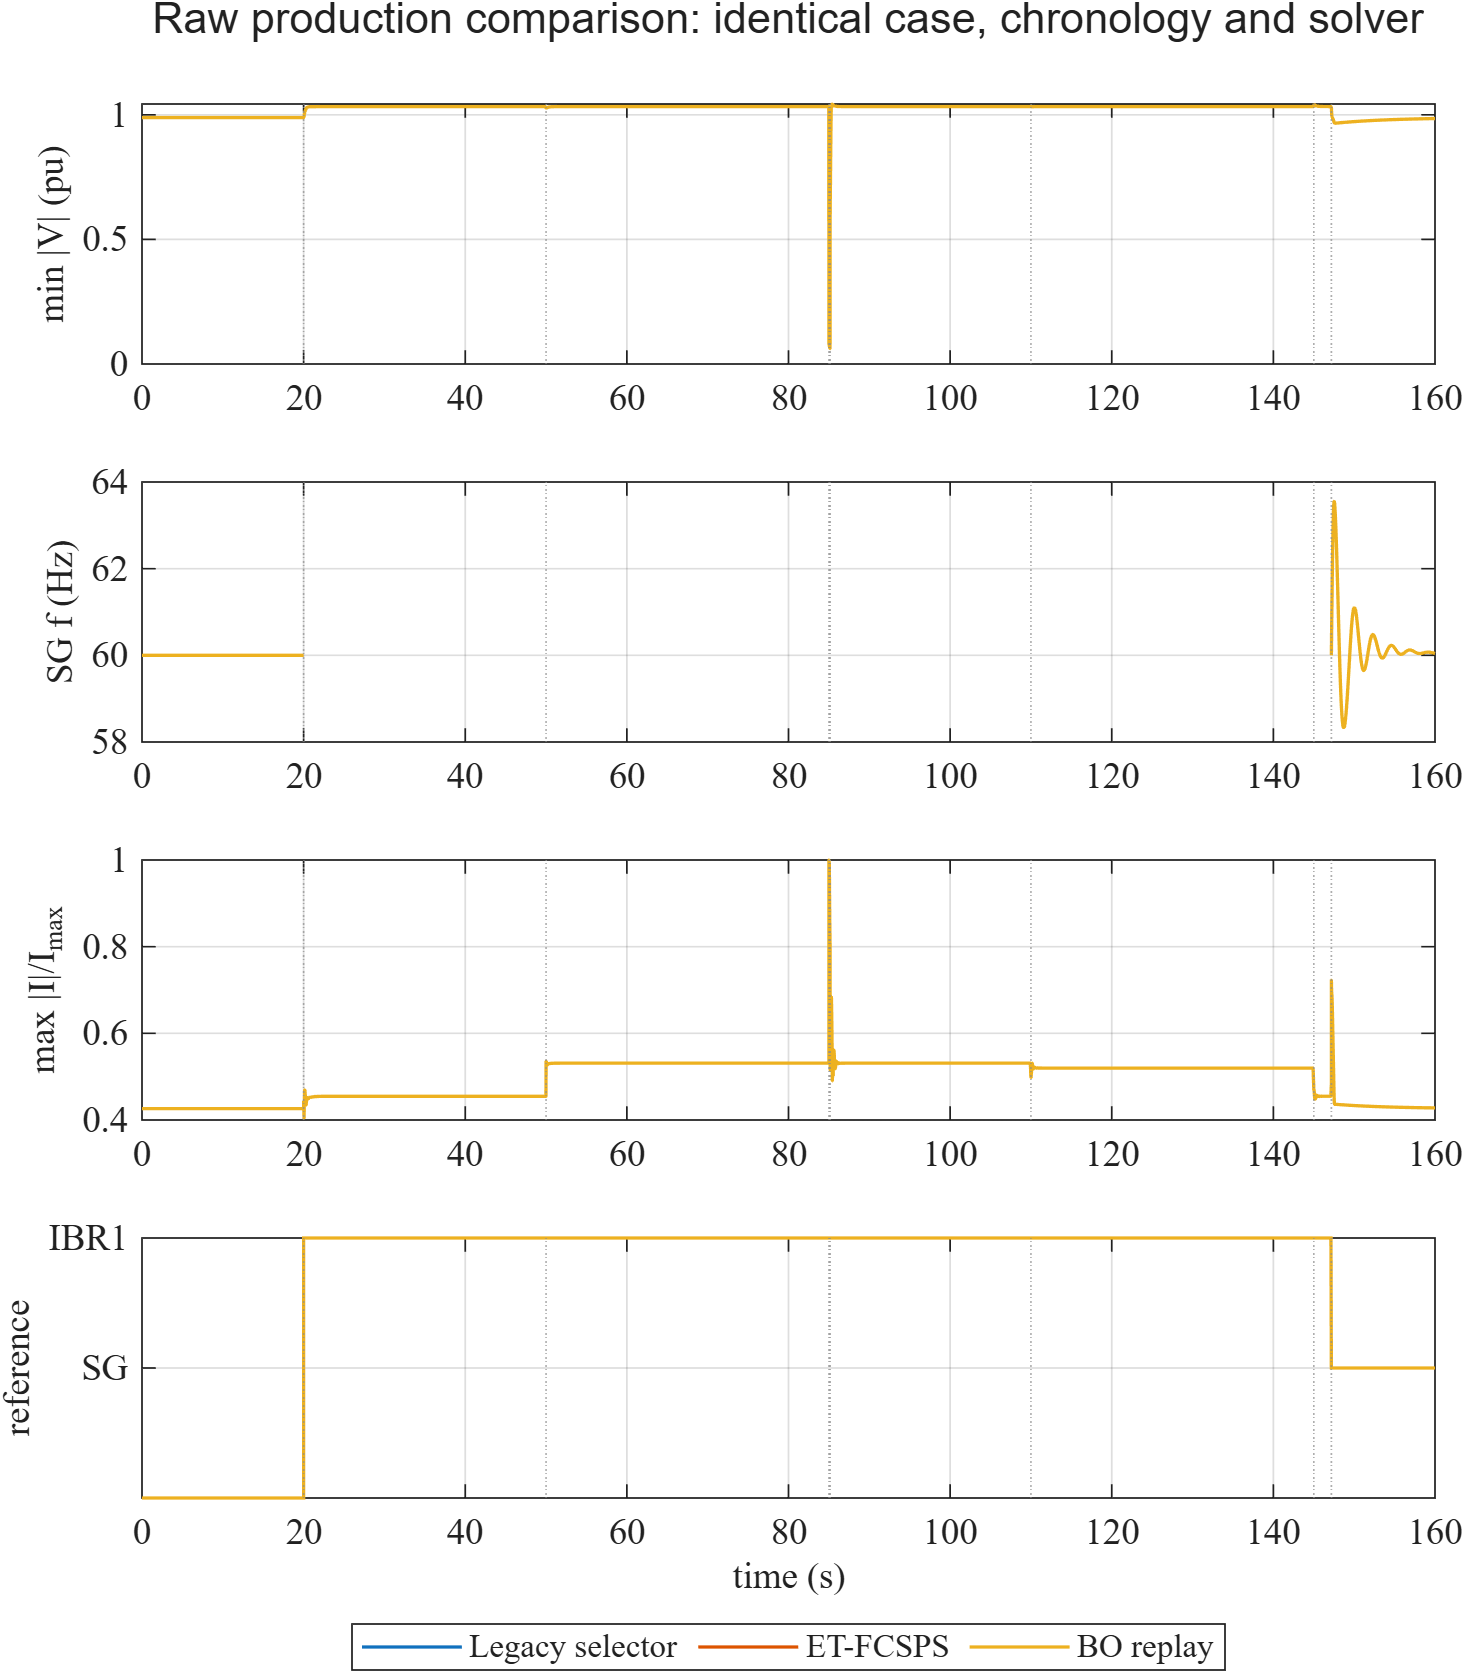
\includegraphics[width=6.4in]{figures/ieee14_controller_compare/controller_comparison_system.png}
\caption{Raw system responses. The three lines coincide because all methods commit the same action.}\end{figure}
\begin{figure}[H]\centering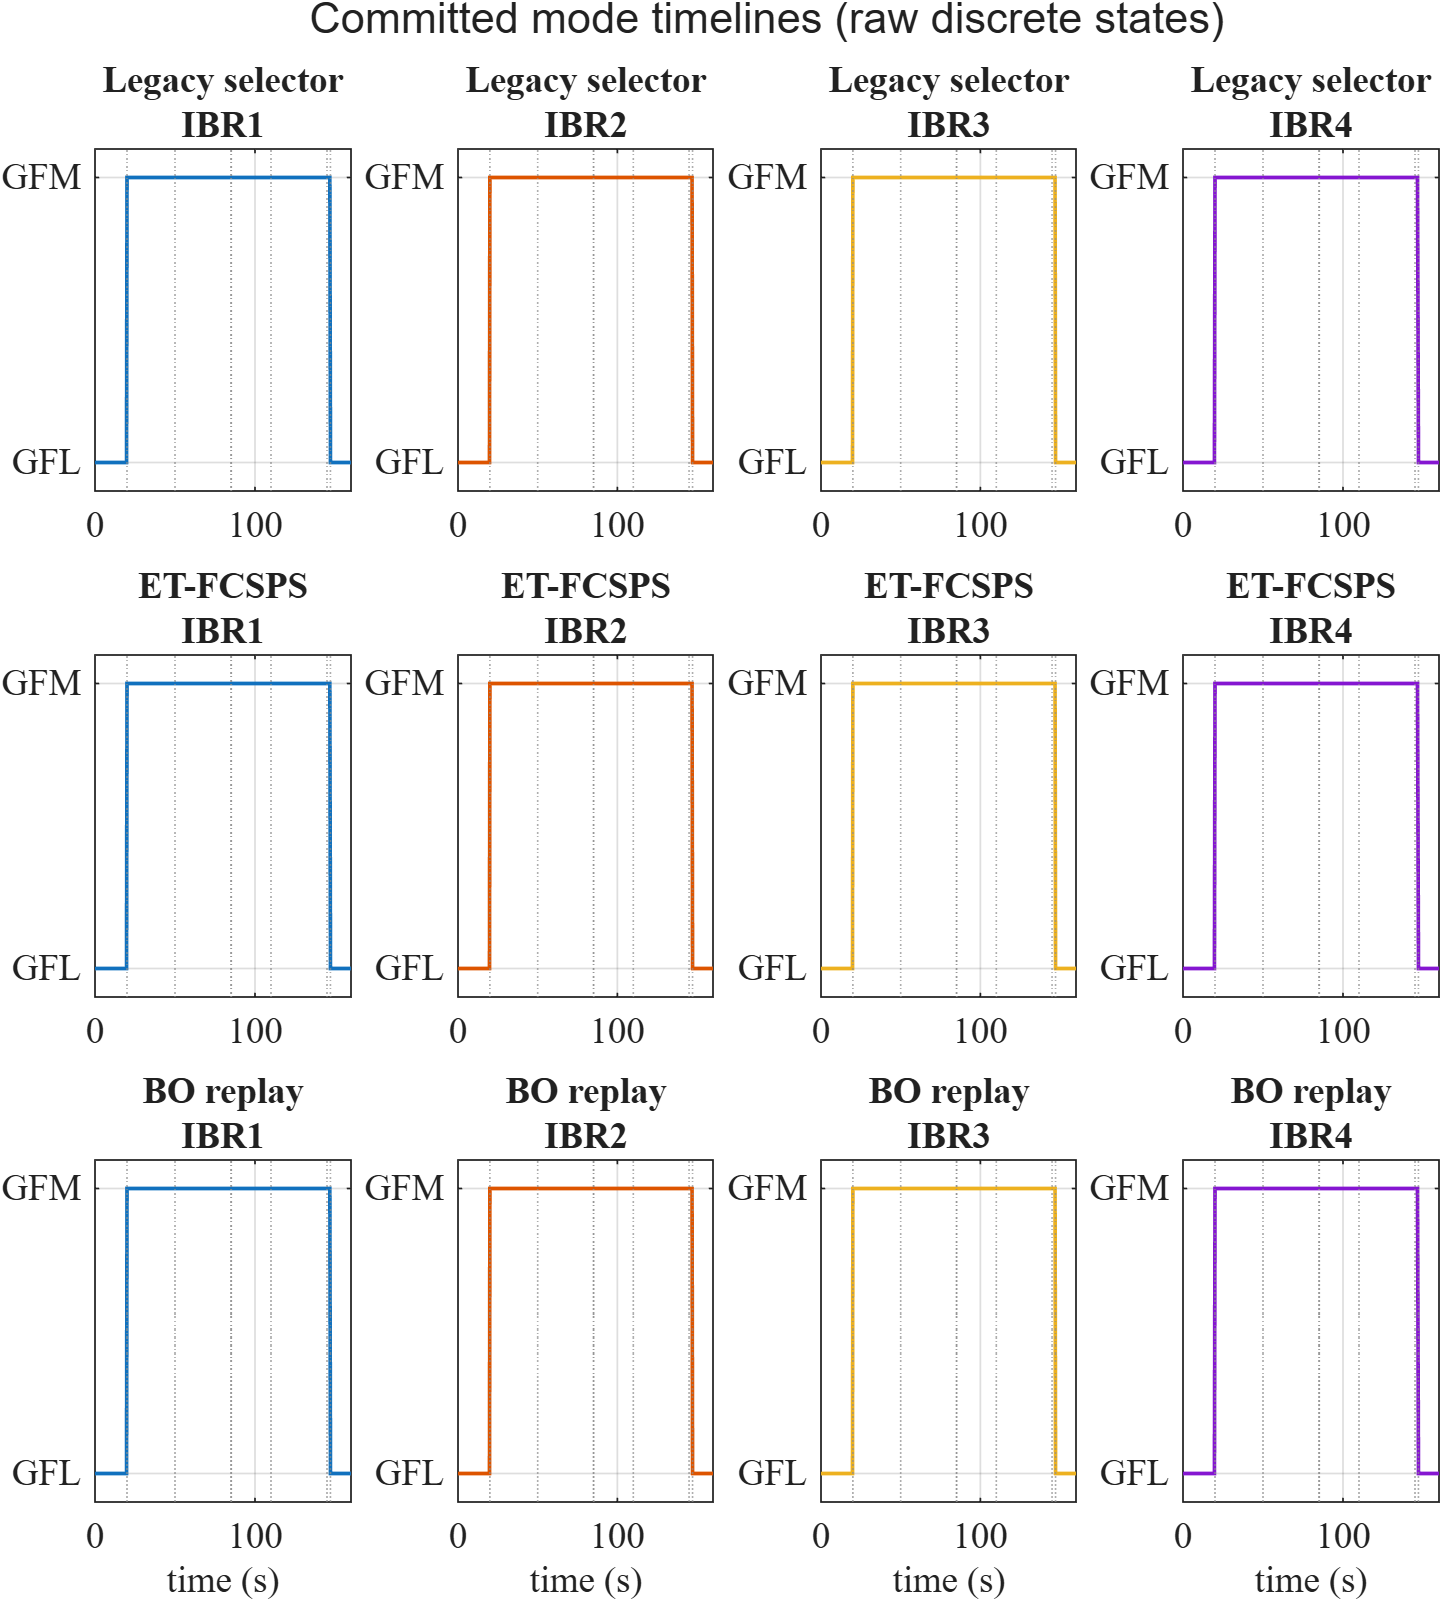
\includegraphics[width=6.4in]{figures/ieee14_controller_compare/controller_comparison_modes.png}
\caption{Committed mode timelines for all four IBRs and all three methods.}\end{figure}
\begin{figure}[H]\centering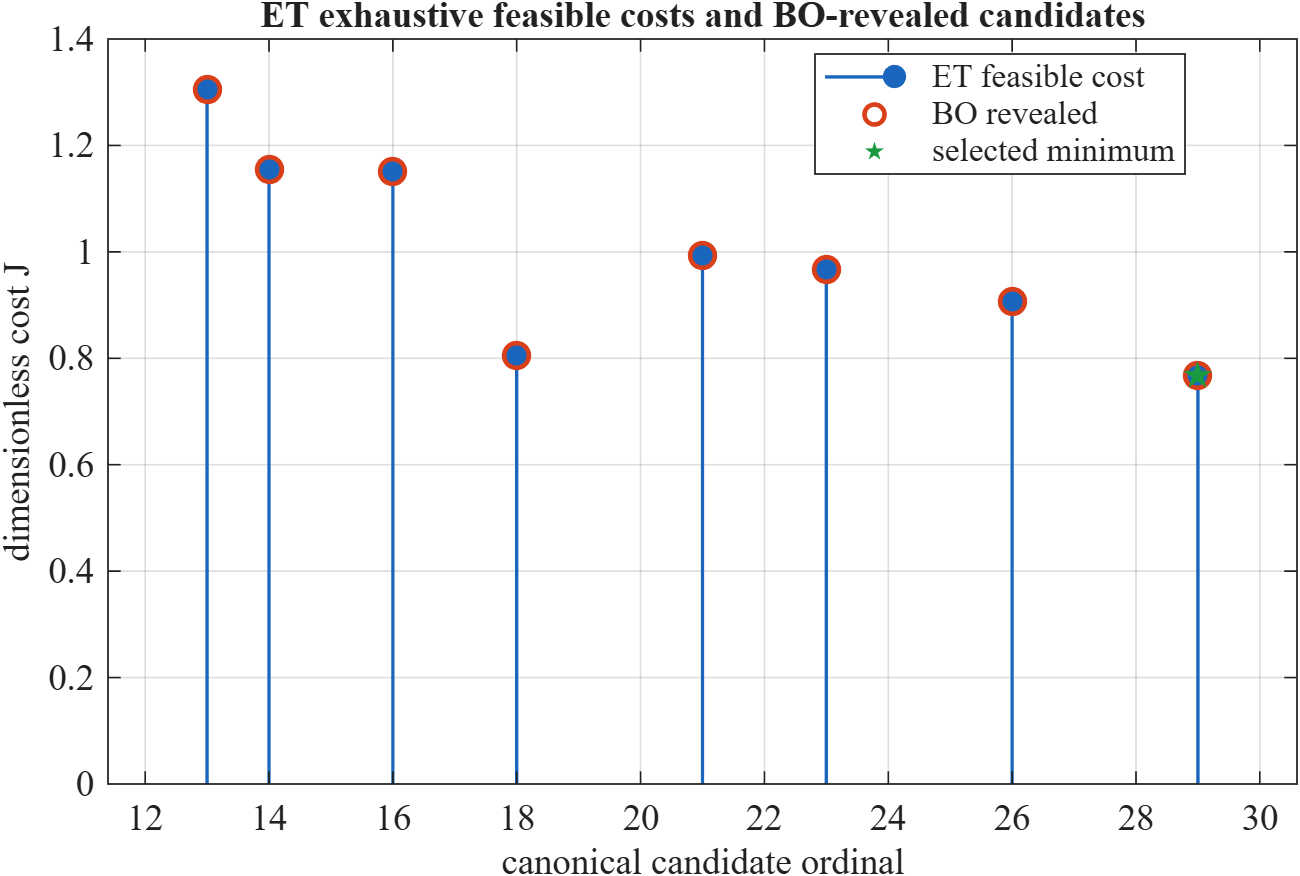
\includegraphics[width=6.4in]{figures/ieee14_controller_compare/controller_candidate_costs.png}
\caption{Eight feasible ET costs and the eight BO-revealed candidates. The BO budget spans the full feasible set.}\end{figure}

\section{Interpretation}
The maximum absolute ET-versus-legacy, BO-versus-legacy, and BO-versus-ET differences are exactly zero for AGSI++, discrete mode, P, Q, $i_d$, $i_q$, frequency, angle, bus voltage, network minimum voltage, reference code, and SG signals. This is expected: the selected discrete action and continuous event-right state are identical, and the production solver is deterministic.

For this case ET-FCSPS is the stronger method. Exhaustive evaluation is tractable, gives a deterministic finite-set global minimum, and introduces no surrogate hyperparameters. BO cannot reduce work because its budget of eight equals the feasible-candidate count. BO may become useful for a larger IBR fleet, but that requires a separate test with a budget below the feasible-set size and measured regret.

The ET and BO long-run wall times were 2182.918 s and 2223.825 s. Their 1.9\% difference is ordinary runtime variation, not a controller benefit, because the dynamic trajectories are identical and common candidate evidence was reused. The historical baseline-cache runtime is not used as a speed benchmark.

\section{Limitations and reproduction}
P/Q reserve uses the existing case-defined nameplate proxy; energy duration and hardware reserve are not established. BO remains offline replay. The result validates this software/controller chronology, not protection, HIL, or field readiness. No equation, threshold, weight, event, solver setting, or raw plot was tuned after viewing the result.

\begin{verbatim}
pf_init_paths;
addpath(fullfile('scripts','reporting'));
out = run_ieee14_controller_comparison(reuse_completed=true);
generate_ieee14_controller_comparison_figures;
\end{verbatim}
\end{document}
